% Name: OSI and TCP/IP layers
% Description: The seven OSI layers beside the four TCP/IP layers they map to, with typical protocols at each level.
% Tags: OSI model, TCP/IP, network layers, protocols

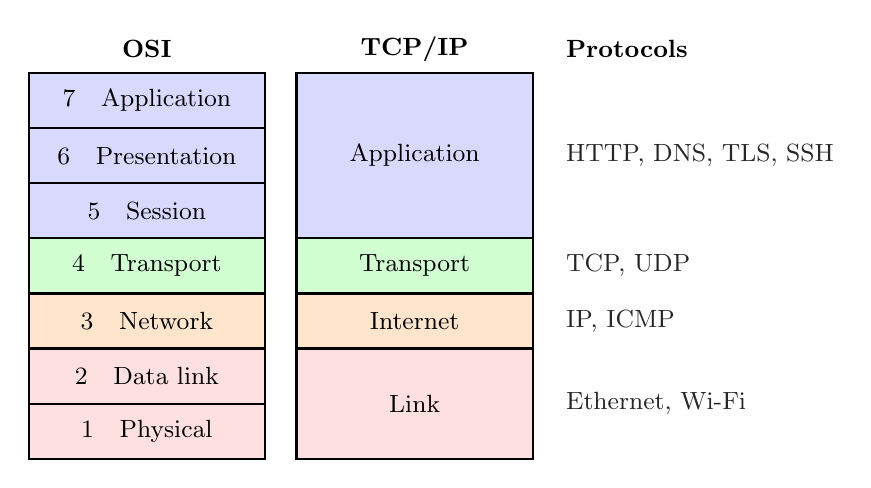
\begin{tikzpicture}[every node/.style={font=\small}, layer/.style={draw, thick, minimum width=30mm, align=center}]
  % Each OSI layer is 0.7 high; layer 7 is at the top.
  \foreach \n/\name/\c in {7/Application/blue!15, 6/Presentation/blue!15, 5/Session/blue!15, 4/Transport/green!18, 3/Network/orange!20, 2/Data link/red!12, 1/Physical/red!12}
    \node[layer, fill=\c, minimum height=7mm] at (0,0.7*\n) {\n\quad \name};
  \foreach \lo/\hi/\name/\c in {5/7/Application/blue!15, 4/4/Transport/green!18, 3/3/Internet/orange!20, 1/2/Link/red!12}
    \node[layer, fill=\c, minimum height={7mm*(\hi-\lo+1)}] at (3.4,{0.35*(\lo+\hi)}) {\name};
  \foreach \lo/\hi/\p in {5/7/{HTTP, DNS, TLS, SSH}, 4/4/{TCP, UDP}, 3/3/{IP, ICMP}, 1/2/{Ethernet, Wi-Fi}}
    \node[anchor=west, gray!30!black] at (5.2,{0.35*(\lo+\hi)}) {\p};
  \node[font=\small\bfseries] at (0,5.55) {OSI};
  \node[font=\small\bfseries] at (3.4,5.55) {TCP/IP};
  \node[font=\small\bfseries, anchor=west] at (5.2,5.55) {Protocols};
\end{tikzpicture}
